\documentclass[tikz,border=3pt]{standalone}

% PGFPlots uses the same text and math fonts as the Typst document.
\usepackage{fontspec}
\usepackage{unicode-math}
\setmainfont{Times New Roman}
\setmathfont[Path=font/]{texgyretermes-math.otf}

\usepackage{pgfplots}
\pgfplotsset{compat=1.18}

\begin{document}
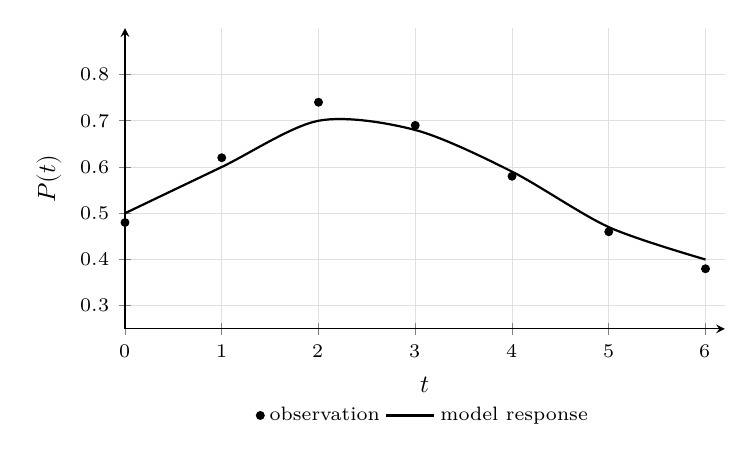
\begin{tikzpicture}
  \begin{axis}[
    width=92mm,
    height=54mm,
    axis lines=left,
    xmin=0, xmax=6.2,
    ymin=0.25, ymax=0.9,
    xtick={0,1,2,3,4,5,6},
    ytick={0.3,0.4,0.5,0.6,0.7,0.8},
    xlabel={$t$},
    ylabel={$P(t)$},
    grid=major,
    grid style={draw=black!12, line width=.35pt},
    tick label style={font=\scriptsize},
    label style={font=\small},
    legend style={draw=none, font=\scriptsize, at={(0.5,-0.22)}, anchor=north,
                  legend columns=2},
  ]
    \addplot+[only marks, color=black, mark=*, mark size=1.4pt,
      mark options={fill=black}]
      coordinates {(0,0.48) (1,0.62) (2,0.74) (3,0.69) (4,0.58) (5,0.46) (6,0.38)};
    \addlegendentry{observation}
    \addplot+[no markers, color=black, line width=.8pt, smooth]
      coordinates {(0,0.50) (1,0.60) (2,0.70) (3,0.68) (4,0.59) (5,0.47) (6,0.40)};
    \addlegendentry{model response}
  \end{axis}
\end{tikzpicture}
\end{document}
